\documentclass[12pt,letterpaper]{article}
\usepackage[utf8]{inputenx} %Codificacion del texto (ISO Latin1 encoding)

\usepackage{fancyhdr} %Permite acomodar a tu gusto la parte de arriba y
% abajo del documento
\usepackage[spanish]{babel} %Permite definir el idioma del dcumento
\usepackage{graphicx} %Permite exportar imagenes en formato eps
\usepackage{url} %Tipo de fuente para correos y paginas
\usepackage{pgf}
\usepackage{fleqn}
\usepackage{amssymb}
\usepackage{amsmath}
\usepackage{fancyvrb}
\usepackage{makeidx}
\usepackage{colortbl} %Permite colocar colores a las tablas
\usepackage{multirow}
\usepackage{booktabs}
\usepackage{moreverb}
\usepackage{rotating}
\usepackage{lastpage}
\usepackage[final]{pdfpages}
%%%%%%%%%%
%Margenes%
%%%%%%%%%%
\usepackage[top=3cm,bottom=3cm,left=3cm,right=3cm,footskip=1.5cm,headheight=1.5cm,headsep=.5cm,textheight=3cm]{geometry}
%%%%%%%%%%%%%%%%%%%%%%
%Estilo del documento%
%%%%%%%%%%%%%%%%%%%%%%
\pagestyle{fancyplain}

%%%%%%%%%%%%%%%%%%%%%%%%%%%%%%%%%%%%%%%%%%%
%Fancyheadings. Top y Bottom del documento%
%%%%%%%%%%%%%%%%%%%%%%%%%%%%%%%%%%%%%%%%%%%
% Recuerde que en este documento la portada del documento no posee
% numeracion, pero de igual manera llamaremos a esa primera pagina la numero
% 1, y la que viene la dos. Esto es para tener una idea de las que
% llamaremos pares e impares
\lhead{Laboratorio mat024} %Parte superior izquierda
\rhead{\bf \it Preinforme 1} %Parte superior derecha
\lfoot{\it Victor Gonzalez} %Parte inferior izquierda. \thepage indica
% el numero de pagina
\cfoot{\bf \thepage} %Parte inferior central
\rfoot{página \thepage\ de \pageref{LastPage}} %Parte inferior derecha
\renewcommand{\footrulewidth}{0.4pt} %Linea de separacion inferior

\begin{document}
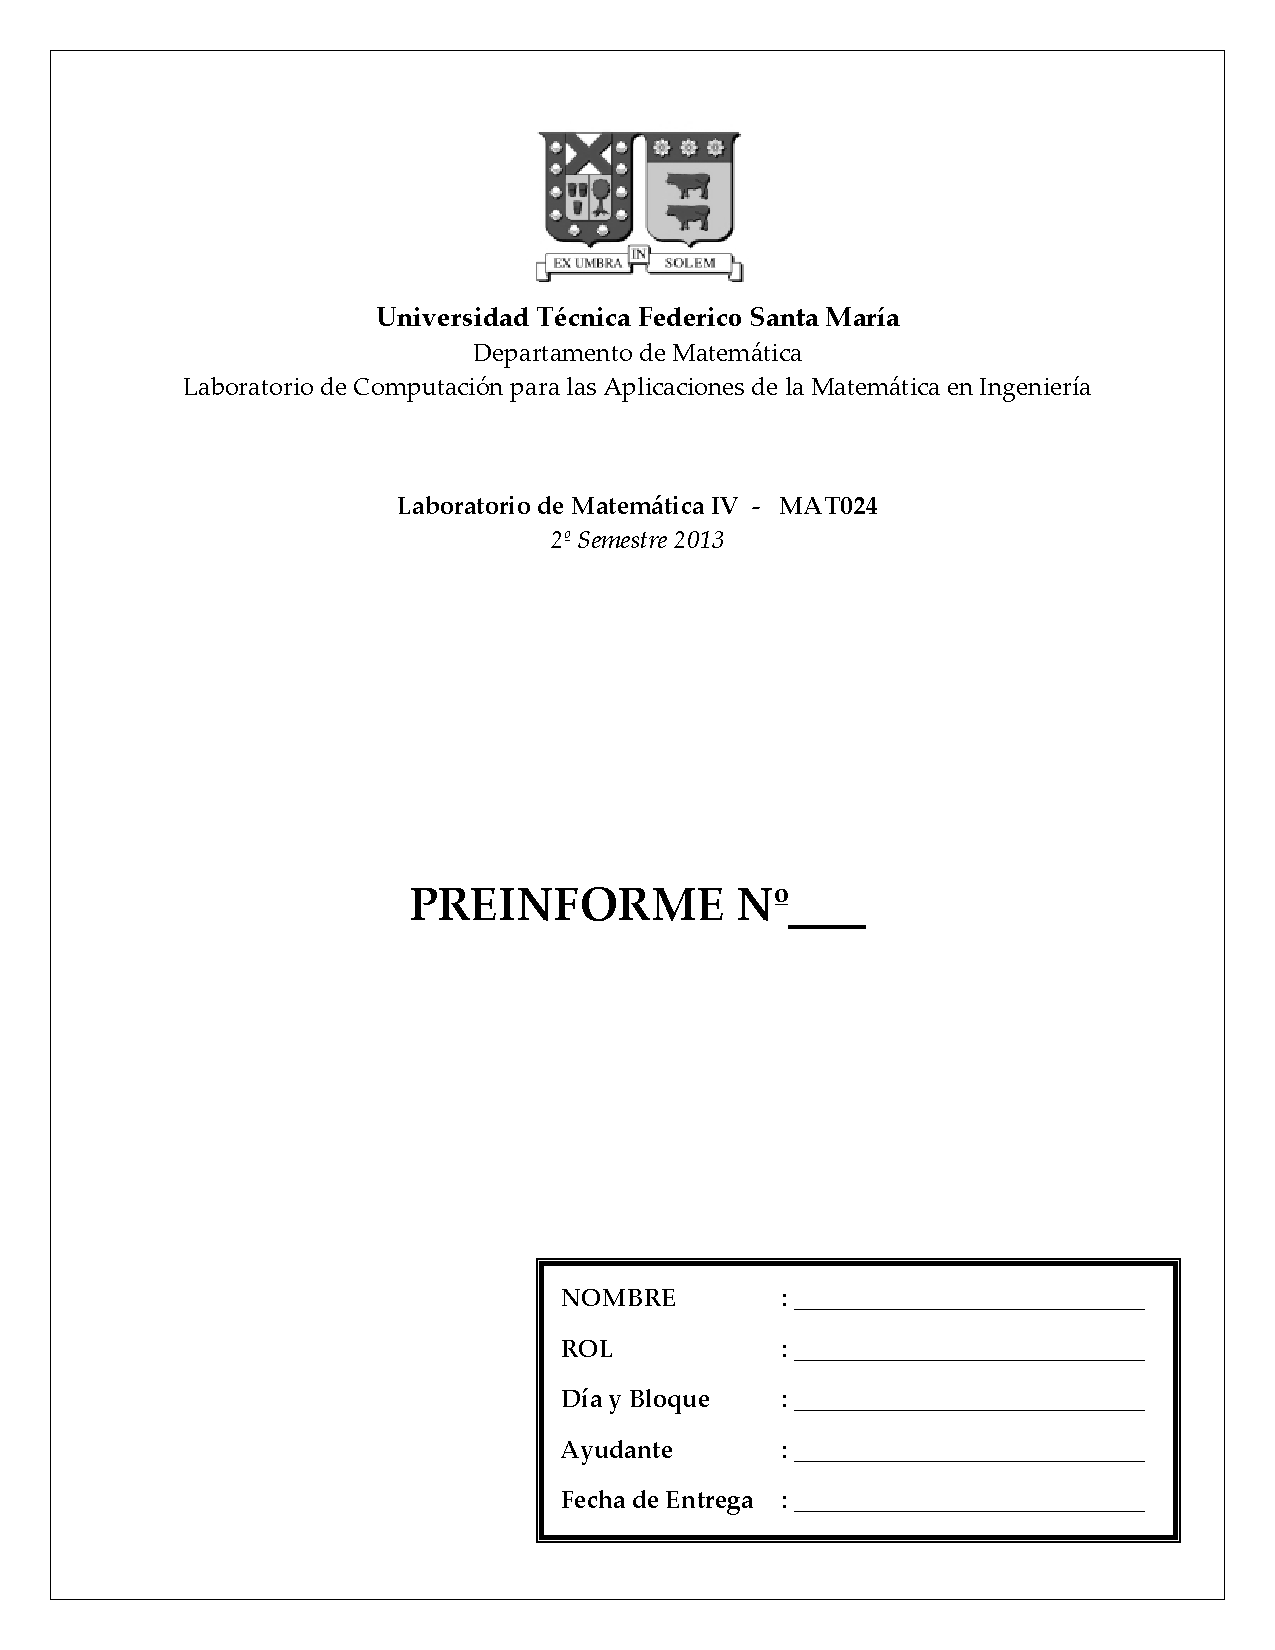
\includepdf[pages={1}]{portada.pdf}

\section{Desarrollo Analítico y Planteamiento}
Para el resto del documento considerar $\alpha=4$ y $\beta=9$.
\subsection{Pregunta 1}
\subsubsection{Parte a}
Se nos pregunta por si la integral $\int\int_Rf(x,y)dA$ existe.

Dado que $f(x,y)=xye^{-\alpha(x^2+y^2)}$ en la región $[0,\beta]$x$[0,\beta]$, es continua y no se indefine de ningún modo, luego por algebra de funciones continuas, la integral existe.

\subsubsection{Parte b}
Se nos pide aproximar mediante Sumas de Riemann, el valor de la integral anteriormente planteada.

Para desarrollar las Sumas de Riemann, se necesita particionar la región a integrar en ``$n$'' particiones. Luego, cada una de estas particiones se irá evaluando en la función que queremos integrar, para luego ser multiplicada por el intervalo. Esto va generando el área o volumen que se quiere integrar.

El procedimiento matemático viene dado por: 
\begin{center}$\sum _{i=1}^n \sum _{j=1}^n (f\left[\frac{x_{i-1}+x_i}{2},\frac{y_{j-1}+y_j}{2}\right]\triangle x \triangle y)$\end{center}

Luego, la aproximación a la integral viene dada por esa suma de Riemann.

\subsubsection{Parte c}
Para obtener el valor exacto de la integral basta calcular: 
\begin{center}$\int_0^{\beta}\int_0^{\beta} xye^{-\alpha(x^2+y^2)} dxdy$\end{center}

El cual en nuestro caso en realidad es:
\begin{center}$\int_0^{9}\int_0^{9} xye^{-4(x^2+y^2)} dxdy$\end{center}

\subsection{Pregunta 2}
\subsubsection{Parte a}
Se nos pide graficar la región $\Omega$ y la imagen bajo la transformación T.

Para graficar $\Omega$, debemos notar que viene delimitada por la función \\$x^{2/5}+y^{2/5}\leq \alpha^{2/5}$, donde además tendremos que $0\leq y\leq x$, es decir, estará delimitado ademas por la función $y\leq x$, la cual cubre la mitad inferior del primer cuadrante.\\

Para graficar $\Omega$ bajo la transformación T, debemos reemplazar la transformación en todas las ecuaciones originales, las cuales nos entregan: $u^{2/5} \leq \alpha^{2/5}$, y ademas $0 \leq uSin^5(v)\leq uCos^5(v)$.

A partir de lo anterior, se obtiene que $0\leq u \leq \alpha$, y $0\leq v \leq \frac{\pi}{4}$.

\subsubsection{Parte b}
Se nos pide calcular la integral: \begin{center}$\int\int_\Omega (\alpha^{2/5}-x^{2/5}-y^{2/5})^2 dA$\end{center}

Pero podemos hacer uso de la conveniente transformación que se utilizó en la parte a, la cual simplificará el cálculo, dejando la integral como:

\begin{center}$\int _0^4\int _0^{\pi /4}(\alpha^{2/5}-u^{2/5})^2 J dvdu$\end{center}

Donde $J$, es el jacobiano de la transformación, el cual viene dado por:
\begin{center}
$J=\left|
\begin{array}{cc}
 \partial _u\left(u*\text{Cos}[v]^5\right) & \partial _u\left(u*\text{Sin}[v]^5\right) \\
 \partial _v\left(u*\text{Cos}[v]^5\right) & \partial _v\left(u*\text{Sin}[v]^5\right) \\
\end{array}
\right|$
\end{center}

\subsubsection{Parte c}
Se nos pide calcular el área de $\Omega$, pero utilizando la transformación, simplificamos el cálculo nuevamente.

\begin{center}$\int\int_\Omega dA = \int\int_{T(\Omega)}JdA$  \end{center}

Lo cual es equivalente a:
\begin{center}$\int _0^4\int _0^{\pi /4}J dvdu$  \end{center}

\section{Desarrollo Computacional}
\subsection{Pregunta 1}
\subsubsection{Parte a}
Se auto-responde en el planteamiento, y se confirma con la gráfica que se puede ver en el anexo\footnote{Notar que la región de la gráfica es menor a la región de integración. Esto se realizó con fines prácticos}.

\subsubsection{Parte b}
Debemos calcular computacionalmente la Suma de Riemann para esta función, la cual viene dada por:
\begin{center}$\sum _{i=1}^n \sum _{j=1}^n (f\left[\frac{x_{i-1}+x_i}{2},\frac{y_{j-1}+y_j}{2}\right]\triangle x \triangle y)$\end{center}

Para esto, hacemos uso de la \textit{Paleta de Herramientas} que nos provee \textit{Mathematica}, para así ingresar facilmente las sumas en el formato visualmente mas conveniente, el cual queda como:

$N\left[\sum _{i=1}^n \sum _{j=1}^n \left(f\left[\frac{x[i-1]+x[i]}{2},\frac{y[j-1]+y[j]}{2}\right]\triangle x \triangle y\right),5\right];$

Todo esto bajo un procedimiento llamado Riemann, el cual fue creado para fines prácticos.
Se crearon además, las sub-funciones $x$ e $y$, las cuales entregan el intervalo de la posición i-ésima.

Para efectos de presentación y orden, se utilizó el comando Grid, para entregar de forma tabulada cada una de los resultados para cada partición junto a su error porcentual.

\subsubsection{Parte c}
Para obtener el valor exacto de la integral: 
\begin{center}$\int_0^{\beta}\int_0^{\beta} xye^{-\alpha(x^2+y^2)} dxdy$\end{center}

Bastó con utilizar la paleta de Mathematica, generando el siguiente comando:
\begin{center}
$N\left[\int _0^{\text{beta}}\int _0^{\text{beta}}f[x,y]dxdy\right]$\end{center}

\subsection{Pregunta 2}
\subsubsection{Parte a}
Para graficar las regiones de integración, nos apoyamos completamente en el comando \textit{RegionPlot}, y en lo encontrado en el planteamiento del ejercicio.

\subsubsection{Parte b y c}
Al igual que en la pregunta 1.c, ingresamos directamente el valor de la integral a Mathematica para que nos entregue un valor numérico.

Adicionalmente, nos apoyamos en la capacidad de cómputo de Mathematica, para obtener el Jacobiano de la transformación.


\section{Resultados}
\subsection{Pregunta 1}
Para cada una de las sumas de Riemann con n=10,50,75 los resultados fueron:

\begin{center}
\begin{tabular}{|c|c|c|}
\hline
 \textbf{n} & \textbf{Valor Obtenido} & \textbf{Error Porcentual} \\ \hline
 10 & 0.032760 & 109.662 \\\hline
 50 & 0.015972 & 2.22296 \\\hline
 75 & 0.015777 & 0.972178 \\\hline
\end{tabular}
\end{center}

Mientras que el resultado real era: 0.015625

\subsection{Pregunta 2}
Las graficas de las regiones $\Omega$ y de la imagen de la transformación pueden verse en el anexo, donde se puede apreciar que $\Omega$ es la region entre la función $y=x$ y la función $xye^{-\alpha(x^2+y^2)}$ del primer cuadrante. Mientras que la imagen de la transformación es un cuadrado.

El resultado de la integral propuesta en la parte b, es 0.106289. El área bajo $\Omega$ resultó ser 0.736311.

\section{Conclusiones}
Las sumas de Riemann son útiles para estimar integrales de dificil cálculo, se limitan a realizar operaciones algebráicas básicas para resolver problemas que pueden ser complejos de entender a nivel de cálculo.
Por otro lado, las transformaciónes de las regiones de integración facilitan enormemente el trabajo del cálculo de integrales en varias variables, y también el análisis de estas, lo cual es ideal.

\includepdf[pages={1,2,3,4}]{lab1_mat.pdf}

\end{document}